\documentclass[aspectratio=43,11pt]{beamer}
\usetheme{default}
\usecolortheme{default}
\setbeamertemplate{navigation symbols}{}
\setbeamertemplate{footline}[frame number]
\setbeamertemplate{itemize items}[circle]
\usepackage{xcolor}
\definecolor{maroon}{HTML}{500000}
\setbeamercolor{structure}{fg=maroon}

\usepackage[T1]{fontenc}
\usepackage{lmodern}
\usepackage{booktabs}
\usepackage{listings}
\usepackage{tikz}
\usetikzlibrary{positioning,arrows.meta}
\lstset{basicstyle=\ttfamily\scriptsize, columns=fullflexible, keepspaces=true,
        showstringspaces=false, breaklines=true}


\title{Mini-Project: Instructions}
\subtitle{data prep $\rightarrow$ ML $\rightarrow$ optimization}
\author{DAEN 300 - Fall 2026}
\date{}
\titlegraphic{\IfFileExists{TAMU_logo.png}{
\includegraphics[height=1.2cm]{TAMU_logo.png}}{}}

\begin{document}

\begin{frame}
  \titlepage
\end{frame}

%===============================================================
\begin{frame}{Goal and timeline}
  \textbf{Goal:} build an end-to-end workflow that predicts
  \begin{itemize}
    \item whether a home was \textbf{inspected} (\texttt{inspnReturned})
    \item whether a household is \textbf{eligible for repair assistance}
          (\texttt{repairAssistanceEligible})
    \item the \textbf{real-property damage} amount (\texttt{rpfvl})
  \end{itemize}
  and shows, with measurements, how you \textbf{optimized} each step.
  \vspace{0.8em}
  \begin{center}
  \begin{tabular}{@{}lll@{}}
    \toprule
    Day & Focus & Deliverable \\
    \midrule
    1 & Explore, understand, plan & Data dictionary + plan \\
    2 & Implement, measure, conclude & Notebook + conclusions \\
    \bottomrule
  \end{tabular}
  \end{center}
\end{frame}

%---------------------------------------------------------------
\begin{frame}[fragile]{Getting the data}

OpenFEMA: IHP Valid Registrations v2
{\tiny\url{https://www.fema.gov/openfema-data-page/individuals-and-households-program-valid-registrations-v2}}

\vspace{0.5em}
          
Work with \textbf{a small set of disasters}!
\end{frame}

%===============================================================
\section{Day 1}

\begin{frame}
  \centering
  \Huge Day 1 \\[0.5em]
  \large Explore $\cdot$ Understand $\cdot$ Plan
\end{frame}

\begin{frame}{Day 1 --- goals}
  By the end of class you should:
  \vspace{0.5em}
  \begin{enumerate}
    \item Load one disaster and record a \textbf{baseline}
          (time, rows, memory)
    \item Know every variable you will use: \textbf{type, meaning, missing values}
    \item Understand the three targets with \textbf{tables and plots}
    \item Decide which fields are \textbf{safe features} (no leakage)
    \item Submit a \textbf{plan}: architecture diagram \emph{and} pseudocode
  \end{enumerate}
\end{frame}

%---------------------------------------------------------------
\begin{frame}{1.1 Load and measure a baseline}
  \begin{itemize}
    \item Load your disaster \textbf{as-is} (default types)
    \item Record:
      \begin{itemize}
        \item download / load time (\texttt{\%time} or \texttt{\%timeit})
        \item number of rows and columns
        \item memory: \texttt{df.memory\_usage(deep=True).sum()}
      \end{itemize}
    \item Keep these numbers --- they are your ``before'' on Day 2
  \end{itemize}
  \vspace{0.8em}
  \begin{center}
  \begin{tabular}{@{}lll@{}}
    \toprule
    Measure & Baseline & After (Day 2) \\
    \midrule
    Load time (s) & & \\
    Rows $\times$ columns & & \\
    Memory (MB) & & \\
    \bottomrule
  \end{tabular}
  \end{center}
\end{frame}

%---------------------------------------------------------------
\begin{frame}{1.2 Build a data dictionary}
  Fill one row per variable you keep:
  \vspace{0.5em}
  \begin{center}
  \footnotesize
  \begin{tabular}{@{}lllll@{}}
    \toprule
    Field & Type & Meaning & \% miss. & Known when? \\
    \midrule
    \texttt{ownRent} & object & O / R / unknown & & registration \\
    \texttt{residenceType} & & & & \\
    \texttt{grossIncome} & & & & \\
    \texttt{inspnReturned} & & & & \\
    \texttt{rpfvl} & & & & after inspection \\
    \dots & & & & \\
    \bottomrule
  \end{tabular}
  \end{center}
  \vspace{0.5em}
  \begin{itemize}
    \item Use the OpenFEMA data page for definitions
    \item ``Known when?'' decides what can be a feature
  \end{itemize}
\end{frame}

%---------------------------------------------------------------
\begin{frame}{1.3 Explore the targets}
  Answer with a table or a plot each:
  \vspace{0.5em}
  \begin{enumerate}
    \item What share of registrations were \textbf{inspected}?
          Of those, what share were \textbf{eligible}?
    \item Are the classes \textbf{balanced}? (affects metric choice)
    \item What does \texttt{rpfvl} look like?
          How many zeros? Histogram of \texttt{rpfvl} and of
          \texttt{np.log1p(rpfvl)}
    \item How do the targets differ by \texttt{ownRent},
          \texttt{residenceType}, \texttt{grossIncome}?
          (use \texttt{groupby})
    \item Anything surprising? Missing codes, odd values, duplicates?
  \end{enumerate}
\end{frame}

%---------------------------------------------------------------
\begin{frame}{1.4 Avoid leakage}
  \textbf{Rule:} a feature must be known \emph{before} the outcome you predict.
  \vspace{0.8em}
  \begin{center}
  \small
  \begin{tabular}{@{}lll@{}}
    \toprule
    Target & Use rows & Safe features \\
    \midrule
    \texttt{inspnReturned} & all registrations & registration fields \\
    \texttt{repairAssistanceEligible} & all (or inspected) & registration fields \\
    \texttt{rpfvl} & inspected only & registration fields \\
    \bottomrule
  \end{tabular}
  \end{center}
  \vspace{0.8em}
  \begin{itemize}
    \item Do \textbf{not} use \texttt{rpfvl} to predict eligibility
    \item Do \textbf{not} use award amounts (\texttt{haAmount}, \dots) as features
    \item Write one sentence justifying each feature you keep
  \end{itemize}
\end{frame}

%---------------------------------------------------------------
\begin{frame}{1.5 Plan: architecture diagram (example)}
  \centering
  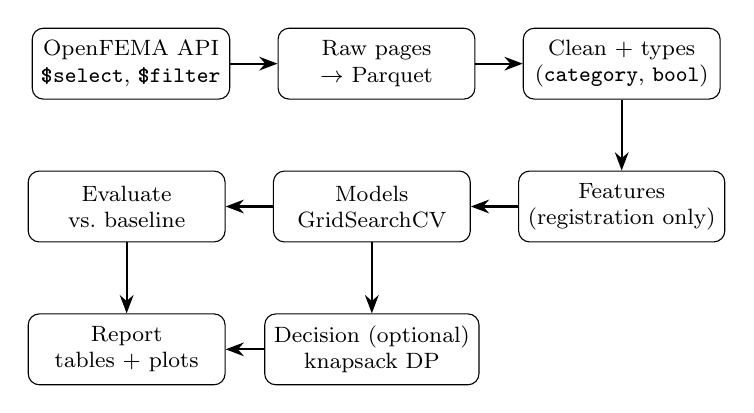
\begin{tikzpicture}[
      box/.style={draw, rounded corners, align=center, minimum width=2.5cm,
                  minimum height=0.9cm, font=\footnotesize},
      arr/.style={-{Stealth}, thick}]
    \node[box] (api) {OpenFEMA API\\\texttt{\$select}, \texttt{\$filter}};
    \node[box, right=0.6cm of api] (raw) {Raw pages\\$\rightarrow$ Parquet};
    \node[box, right=0.6cm of raw] (clean) {Clean + types\\(\texttt{category}, \texttt{bool})};
    \node[box, below=0.9cm of clean] (feat) {Features\\(registration only)};
    \node[box, left=0.6cm of feat] (ml) {Models\\GridSearchCV};
    \node[box, left=0.6cm of ml] (eval) {Evaluate\\vs.\ baseline};
    \node[box, below=0.9cm of ml] (dec) {Decision (optional)\\knapsack DP};
    \node[box, below=0.9cm of eval] (rep) {Report\\tables + plots};
    \draw[arr] (api) -- (raw);
    \draw[arr] (raw) -- (clean);
    \draw[arr] (clean) -- (feat);
    \draw[arr] (feat) -- (ml);
    \draw[arr] (ml) -- (eval);
    \draw[arr] (ml) -- (dec);
    \draw[arr] (eval) -- (rep);
    \draw[arr] (dec) -- (rep);
  \end{tikzpicture}\par
  \vspace{0.8em}
  \raggedright
  \small Draw \emph{your own}: mark where you will \textbf{measure} time or memory.
\end{frame}

%---------------------------------------------------------------
\begin{frame}[fragile]{1.6 Plan: pseudocode (template)}
\begin{lstlisting}
FUNCTION fetch(disaster, columns):
    rows <- empty;  skip <- 0
    REPEAT
        page <- API(select=columns, filter=disaster, top=10000, skip=skip)
        append page to rows;  skip <- skip + 10000
    UNTIL page is empty
    SAVE rows as parquet

FUNCTION prepare(df):
    set dtypes (category, bool, float32);  handle missing codes
    RETURN features X (registration fields), targets y1, y2, y3

FOR each target in [inspnReturned, repairAssistanceEligible, rpfvl]:
    split train / test
    fit BASELINE;  record score
    GridSearchCV(model, grid);  record best params, test score
    plot validation curve

REPORT before/after table, plots, conclusions
\end{lstlisting}
\end{frame}

%---------------------------------------------------------------
\begin{frame}{Day 1 --- deliverable}
  Submit on Canvas (notebook or PDF):
  \vspace{0.5em}
  \begin{itemize}
    \item[$\square$] Baseline table: time, rows, memory
    \item[$\square$] Data dictionary for every field you keep
    \item[$\square$] 3--5 exploratory tables/plots with one-line takeaways
    \item[$\square$] Feature list with a leakage check
    \item[$\square$] Architecture diagram (hand-drawn photo is fine, or draw.io)
    \item[$\square$] Pseudocode or algorithm for the full workflow
    \item[$\square$] What you expect to optimize, and how you will measure it
  \end{itemize}
\end{frame}

%===============================================================
\section{Day 2}

\begin{frame}
  \centering
  \Huge Day 2 \\[0.5em]
  \large Implement $\cdot$ Measure $\cdot$ Conclude
\end{frame}

\begin{frame}{Day 2 --- goals}
  By the end of class you should:
  \vspace{0.5em}
  \begin{enumerate}
    \item Implement your Day 1 plan (update it if it changed)
    \item Show \textbf{before vs.\ after} for the data pipeline and code
    \item Train, tune, and evaluate models against a \textbf{baseline}
    \item (Optional) turn predictions into a \textbf{decision}
    \item Write \textbf{conclusions} supported by your numbers
  \end{enumerate}
\end{frame}

%---------------------------------------------------------------
\begin{frame}{2.1 Optimize the pipeline and the code}
  \textbf{Pipeline}
  \begin{itemize}
    \item Fetch only needed columns and rows; load with
          \texttt{usecols}, \texttt{dtype}, \texttt{chunksize}
    \item Convert codes to \texttt{category}, flags to \texttt{bool}
    \item Fill the ``After'' column of your Day 1 baseline table
  \end{itemize}
  \vspace{0.5em}
  \textbf{Code}
  \begin{itemize}
    \item Profile one slow step with \texttt{\%prun}
    \item Replace a loop or \texttt{.apply()} with a vectorized version
          or \texttt{groupby}
    \item Report $\text{speedup} = t_{\text{before}} / t_{\text{after}}$
  \end{itemize}
\end{frame}

%---------------------------------------------------------------
\begin{frame}{2.2 Optimize the models}
  For each target:
  \vspace{0.3em}
  \begin{itemize}
    \item \textbf{Baseline}: majority class (classification) or mean (regression)
    \item \textbf{Model}: e.g., logistic regression / decision tree / random forest
    \item \textbf{Tune} with \texttt{GridSearchCV} (cross-validation on training set only)
    \item \textbf{Validation curve} for one hyperparameter
    \item \textbf{Evaluate} once on the test set
  \end{itemize}
  \vspace{0.5em}
  \begin{center}
  \footnotesize
  \begin{tabular}{@{}lll@{}}
    \toprule
    Target & Metric & Tip \\
    \midrule
    \texttt{inspnReturned} & F1, confusion matrix & check class balance \\
    \texttt{repairAssistanceEligible} & F1, confusion matrix & same \\
    \texttt{rpfvl} & RMSE, MAE & try \texttt{np.log1p} \\
    \bottomrule
  \end{tabular}
  \end{center}
\end{frame}

%---------------------------------------------------------------
\begin{frame}{2.3 Conclusions}
  Answer in short paragraphs, each backed by a number, table, or plot:
  \vspace{0.5em}
  \begin{enumerate}
    \item Which optimization gave the \textbf{largest gain}, and why?
    \item How much better than the \textbf{baseline} is each model?
    \item Which features mattered most? Does that make sense?
    \item What are the \textbf{limitations}? (one disaster, missing data,
          human error in raw records)
    \item What would you do with \textbf{more time or more data}?
  \end{enumerate}
\end{frame}

%---------------------------------------------------------------
\begin{frame}{Day 2 --- final deliverable}
  Submit on Canvas: one Jupyter notebook (and its PDF export)
  \vspace{0.5em}
  \begin{itemize}
    \item[$\square$] Updated plan (diagram + pseudocode), noting any changes
    \item[$\square$] Before/after table: time, memory, speedup
    \item[$\square$] Model results vs.\ baseline, with validation curves
    \item[$\square$] Conclusions
    \item[$\square$] Sources and AI use acknowledged
  \end{itemize}
  \vspace{0.8em}
  \small Presentation quality --- organization, clarity, tables, graphs,
  discussion --- is part of the grade.
\end{frame}

\end{document}
